\documentclass{standalone}
\usepackage{tikz}
\usetikzlibrary{positioning, shapes.geometric, arrows.meta, calc,matrix}

\begin{document}

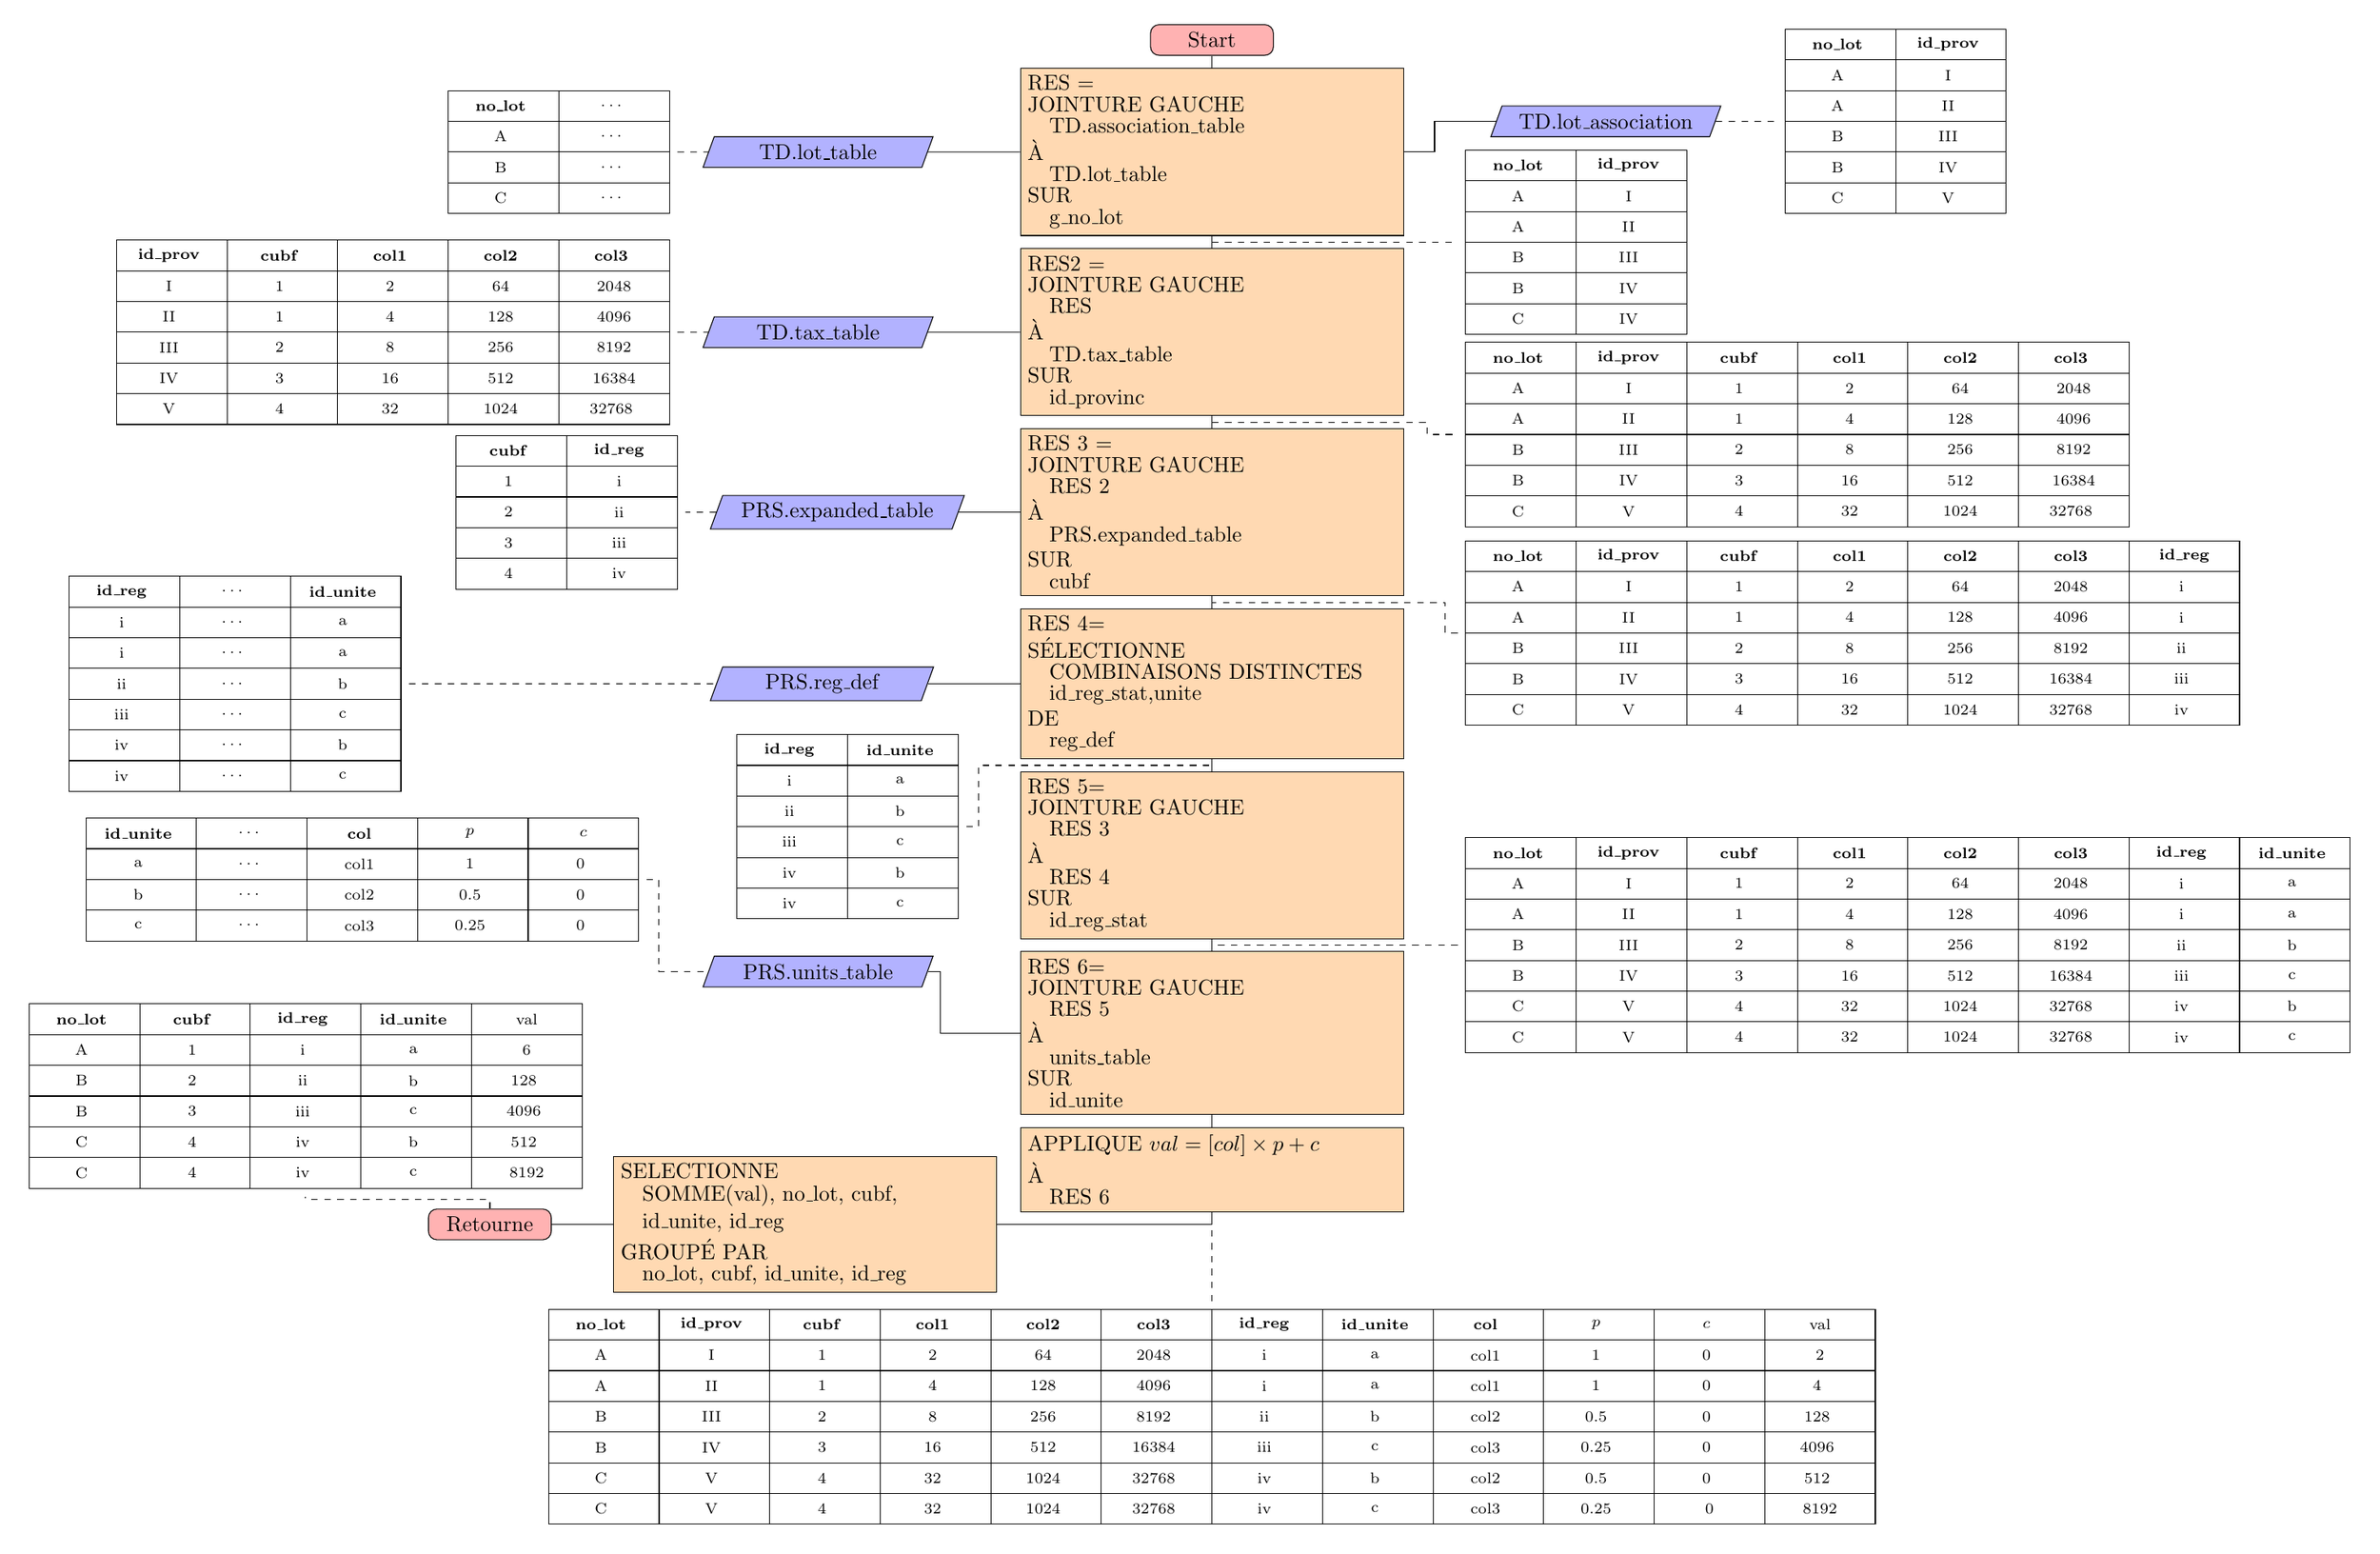
\begin{tikzpicture}[
    table/.style={rectangle, draw, minimum width=4cm, minimum height=1.5cm, text centered, fill=blue!10},
    startstop/.style={rectangle, rounded corners, minimum width=2cm, minimum height=0.5cm,text centered, draw=black, fill=red!30},
    io/.style={trapezium, trapezium left angle=70, trapezium right angle=110, minimum width=1.5cm, minimum height=0.5cm, text centered, draw=black, fill=blue!30,text width=3cm},
    process/.style={rectangle, minimum width=2cm, minimum height=0.5cm, text centered, draw=black, fill=orange!30,align=left,text width=6cm},
    decision/.style={diamond, minimum width=3cm, text centered, draw=black, fill=green!30, aspect=2},
    arrow/.style={thick,->,>=stealth}
]

% Nodes
\node[startstop] (deb) {Start};
% op 1
\node[process, below=0.2cm of deb,align=left] (merge_lot_data) {\shortstack[l]{RES = \\JOINTURE GAUCHE \\\quad TD.association\_table \\À \\ \quad TD.lot\_table \\ SUR \\ \quad g\_no\_lot}};
\node[io, left=1.5cm of merge_lot_data] (td_lot) {TD.lot\_table};
\node[io,right=1.5cm of merge_lot_data,yshift=0.5cm](td-assoc){TD.lot\_association};
\matrix (lot-table) [matrix of nodes,
                  nodes in empty cells,
                  nodes={draw, minimum width=1.8cm, minimum height=0.5cm, align=left, anchor=west, font=\scriptsize},
                  column sep=-\pgflinewidth, row sep=-\pgflinewidth,
                  left=0.5cm of td_lot] {
    \textbf{no\_lot}  & $\cdots$  \\
    A                     & $\cdots$  \\
    B                     & $\cdots$ \\
    C                     & $\cdots$ \\
};

\matrix (lot-assoc-table) [matrix of nodes,
                  nodes in empty cells,
                  nodes={draw, minimum width=1.8cm, minimum height=0.5cm, align=left, anchor=east, font=\scriptsize},
                  column sep=-\pgflinewidth, row sep=-\pgflinewidth,
                  right=1cm of td-assoc] {
    \textbf{no\_lot}   & \textbf{id\_prov} \\
    A                     & I     \\
    A                     & II    \\
    B                     & III   \\
    B                     & IV    \\
    C                     & V     \\
};


% op 2
\node[process, below=0.2cm of merge_lot_data, align=left] (merge_tax) {\shortstack[l]{RES2 = \\JOINTURE GAUCHE \\\quad RES \\À \\ \quad TD.tax\_table\\ SUR \\ \quad id\_provinc}};
\node[io, left=1.5cm of merge_tax] (td_tax) {\shortstack{TD.tax\_table}};
\coordinate (step1) at ($(merge_lot_data.south)!0.5!(merge_tax.north)$);
\matrix (res) [matrix of nodes,
                  nodes in empty cells,
                  nodes={draw, minimum width=1.8cm, minimum height=0.5cm, align=left, anchor=west, font=\scriptsize},
                  column sep=-\pgflinewidth, row sep=-\pgflinewidth,
                  right=4cm of step1] {
    \textbf{no\_lot}     & \textbf{id\_prov} \\
    A                 & I    \\
    A                 & II   \\
    B                 & III  \\
    B                 & IV   \\  
    C                 & IV   \\
};
\matrix (tax-table-actual) [matrix of nodes,
                  nodes in empty cells,
                  nodes={draw, minimum width=1.8cm, minimum height=0.5cm, align=left, anchor=west, font=\scriptsize},
                  column sep=-\pgflinewidth, row sep=-\pgflinewidth,
                  left=0.5cm of td_tax] {
    \textbf{id\_prov} & \textbf{cubf}   & \textbf{col1} & \textbf{col2} & \textbf{col3} \\
    I                 & 1               & 2             & 64             & 2048\\
    II                & 1               & 4             & 128             & 4096\\
    III               & 2               & 8             & 256             & 8192\\
    IV                & 3               & 16             & 512             & 16384\\
    V                 & 4               & 32             & 1024           & 32768 \\
};
% op3 
\node[process,below=0.2cm of merge_tax,align=left](merge_reg){\shortstack[l]{RES 3 = \\JOINTURE GAUCHE \\\quad RES 2 \\À \\ \quad PRS.expanded\_table\\ SUR \\ \quad cubf}};
\node[io, left=1cm of merge_reg,text width=3.5cm] (reg-tax-assoc) {PRS.expanded\_table};
\coordinate (step2) at ($(merge_tax.south)!0.5!(merge_reg.north)$);
\matrix (res2) [matrix of nodes,
                  nodes in empty cells,
                  nodes={draw, minimum width=1.8cm, minimum height=0.5cm, align=left, anchor=west, font=\scriptsize},
                  column sep=-\pgflinewidth, row sep=-\pgflinewidth,
                  right=4cm of step2,yshift=-0.2cm] {
    \textbf{no\_lot}   & \textbf{id\_prov} & \textbf{cubf}   & \textbf{col1} & \textbf{col2} & \textbf{col3} \\                     
    A                 & I                 & 1               & 2             & 64             & 2048\\
    A                 & II                & 1               & 4             & 128            & 4096\\
    B                & III               & 2               & 8             & 256            & 8192\\
    B                 & IV                & 3               & 16            & 512            & 16384\\
    C                 & V                & 4               & 32             & 1024           & 32768 \\
};
\matrix (cubf-id-assoc-actual) [matrix of nodes,
                  nodes in empty cells,
                  nodes={draw, minimum width=1.8cm, minimum height=0.5cm, align=left, anchor=west, font=\scriptsize},
                  column sep=-\pgflinewidth, row sep=-\pgflinewidth,
                  left=0.5cm of reg-tax-assoc] {
    \textbf{cubf}  &  \textbf{id\_reg}  \\                     
    1                 & i               \\
    2                 & ii               \\
    3                 & iii               \\
    4                 & iv               \\};
%op 4
\node[process,below=0.2cm of merge_reg,text width = 6cm,align=left] (distinct-unit-rules){\shortstack[l]{RES 4=\\SÉLECTIONNE\\ \quad COMBINAISONS DISTINCTES \\\quad id\_reg\_stat,unite\\ DE\\ \quad reg\_def}};
\node[io, left=1.5cm of distinct-unit-rules] (reg-def) {PRS.reg\_def};
\coordinate (step3) at ($(merge_reg.south)!0.5!(distinct-unit-rules.north)$);
\matrix (res3) [matrix of nodes,
                  nodes in empty cells,
                  nodes={draw, minimum width=1.8cm, minimum height=0.5cm, align=left, anchor=west, font=\scriptsize},
                  column sep=-\pgflinewidth, row sep=-\pgflinewidth,
                  right=4cm of step3,yshift=-0.5cm] {
    \textbf{no\_lot}  & \textbf{id\_prov} & \textbf{cubf}   & \textbf{col1} & \textbf{col2} & \textbf{col3} &  \textbf{id\_reg}\\                     
    A                 & I                 & 1               & 2             & 64              & 2048            &   i          \\
    A                 & II                & 1               & 4             & 128             & 4096            &   i      \\
    B                 & III               & 2               & 8             & 256             & 8192            &   ii      \\
    B                 & IV                & 3               & 16            & 512             & 16384          &   iii      \\
    C                 &  V                & 4               & 32            & 1024            & 32768            &   iv        \\
};

\matrix (reg-def-actual) [matrix of nodes,
                  nodes in empty cells,
                  nodes={draw, minimum width=1.8cm, minimum height=0.5cm, align=left, anchor=west, font=\scriptsize},
                  column sep=-\pgflinewidth, row sep=-\pgflinewidth,
                  left=5cm of reg-def] {
    \textbf{id\_reg}  & $\cdots$ & \textbf{id\_unite}     \\                     
    i                 & $\cdots$ & a                    \\
    i                 & $\cdots$ & a                    \\
    ii                & $\cdots$ & b                    \\
    iii               & $\cdots$ & c                    \\
    iv                & $\cdots$ & b                     \\
    iv                & $\cdots$ & c                     \\};


%op 5
\node[process,below=0.2cm of distinct-unit-rules, align=left](jointure-reg-unite){\shortstack[l]{\shortstack[l]{RES 5=\\JOINTURE GAUCHE\\ \quad RES 3 \\À \\\quad RES 4 \\ SUR \\\quad id\_reg\_stat}}};
% data values op 4
\coordinate (step4) at ($(distinct-unit-rules.south)!0.5!(jointure-reg-unite.north)$);
\matrix (res4) [matrix of nodes,
                  nodes in empty cells,
                  nodes={draw, minimum width=1.8cm, minimum height=0.5cm, align=left, anchor=west, font=\scriptsize},
                  column sep=-\pgflinewidth, row sep=-\pgflinewidth,
                  left=4cm of step4,yshift=-1cm] {
    \textbf{id\_reg}   & \textbf{id\_unite}     \\                     
    i                  & a                    \\
    ii                 & b                    \\
    iii                & c                    \\
    iv                 & b                     \\
    iv                 & c                     \\};
%op 6
\node[process,below=0.2cm of jointure-reg-unite, align=left](join-unite-convers){\shortstack[l]{\shortstack[l]{RES 6=\\JOINTURE GAUCHE\\ \quad RES 5 \\À \\\quad units\_table \\ SUR \\\quad id\_unite}}};
\node[io, left=1.5cm of join-unite-convers,yshift=1cm] (unites-def) {PRS.units\_table};
\matrix (convers-fact-actual) [matrix of nodes,
                  nodes in empty cells,
                  nodes={draw, minimum width=1.8cm, minimum height=0.5cm, align=left, anchor=west, font=\scriptsize},
                  column sep=-\pgflinewidth, row sep=-\pgflinewidth,
                  left=1cm of unites-def,yshift = 1.5cm] {
    \textbf{id\_unite}  & $\cdots$ & \textbf{col}     & $p$ & $c$\\                     
    a                 & $\cdots$ & col1               & 1   & 0   \\
    b                 & $\cdots$ & col2               & 0.5 & 0    \\
    c                 & $\cdots$ & col3               & 0.25 & 0     \\};
% data value op 5
\coordinate (step5) at ($(jointure-reg-unite.south)!0.5!(join-unite-convers.north)$);
\matrix (res5) [matrix of nodes,
                  nodes in empty cells,
                  nodes={draw, minimum width=1.8cm, minimum height=0.5cm, align=left, anchor=west, font=\scriptsize},
                  column sep=-\pgflinewidth, row sep=-\pgflinewidth,
                  right=4cm of step5] {
    \textbf{no\_lot}  & \textbf{id\_prov} & \textbf{cubf}   & \textbf{col1} & \textbf{col2} & \textbf{col3} &  \textbf{id\_reg} & \textbf{id\_unite} \\                     
    A                & I                 & 1               & 2             & 64              & 2048            &   i      & a  \\
    A                 & II                & 1               & 4             & 128             & 4096            &   i      & a  \\
    B                 & III               & 2               & 8             & 256             & 8192            &   ii     & b  \\
    B                 & IV                & 3               & 16            & 512             & 16384           &   iii    & c  \\
    C                 &  V                & 4               & 32            & 1024            & 32768           &   iv    & b   \\
    C                 &  V                & 4               & 32            & 1024            & 32768           &   iv    & c   \\
};



%op 7
\node[process,below=0.2cm of join-unite-convers, align=left](unite-convers){\shortstack[l]{\shortstack[l]{APPLIQUE $val =[col]\times p +c$\\À \\\quad RES 6}}};

% op 8
\coordinate (step6) at ($(unite-convers.south)+(0,-0.2)$);
\node[process,left=3.5cm of step6, align=left](aggreg){\shortstack[l]{\shortstack[l]{SELECTIONNE \\ \quad SOMME(val), no\_lot, cubf, \\ \quad id\_unite, id\_reg \\ GROUPÉ PAR \\ \quad no\_lot, cubf, id\_unite, id\_reg}}};

% data value op 7

\matrix (applique-actual) [matrix of nodes,
                  nodes in empty cells,
                  nodes={draw, minimum width=1.8cm, minimum height=0.5cm, align=left, anchor=west, font=\scriptsize},
                  column sep=-\pgflinewidth, row sep=-\pgflinewidth,
                  below=1.25cm of step6] {
    \textbf{no\_lot}    & \textbf{id\_prov}   & \textbf{cubf}   & \textbf{col1} & \textbf{col2} & \textbf{col3} &  \textbf{id\_reg} & \textbf{id\_unite}    & \textbf{col}  & $p$ & $c$ & val\\                        
    A                   & I                   & 1               & 2             & 64              & 2048            &   i             & a                     & col1          & 1   & 0 &  2\\
    A                   & II                  & 1               & 4             & 128             & 4096            &   i             & a                     & col1          & 1   & 0  & 4 \\
    B                   & III                 & 2               & 8             & 256             & 8192            &   ii            & b                     & col2          & 0.5 & 0  & 128  \\
    B                   & IV                  & 3               & 16            & 512             & 16384           &   iii           & c                     & col3          & 0.25 & 0 & 4096 \\
    C                   &  V                  & 4               & 32            & 1024            & 32768           &   iv            & b                     & col2          & 0.5 & 0 & 512 \\
    C                   &  V                  & 4               & 32            & 1024            & 32768           &   iv            & c                     & col3          & 0.25 & 0& 8192\\
};
\node[startstop,left=1cm of aggreg](fin){Retourne};
\matrix (resultat-final) [matrix of nodes,
                  nodes in empty cells,
                  nodes={draw, minimum width=1.8cm, minimum height=0.5cm, align=left, anchor=south east, font=\scriptsize},
                  column sep=-\pgflinewidth, row sep=-\pgflinewidth,
                  above=0.2cm of fin,xshift=-3cm] {
    \textbf{no\_lot}    & \textbf{cubf}   &  \textbf{id\_reg} & \textbf{id\_unite}  & val\\                        
    A                   & 1               &   i             & a                     &  6\\
    B                   & 2               &   ii            & b                     & 128  \\
    B                   & 3               &   iii           & c                     & 4096 \\
    C                   & 4               &   iv            & b                     & 512 \\
    C                   & 4               &   iv            & c                     & 8192\\
};
% Logic arrows
\draw (deb) -- (merge_lot_data);
\draw (merge_lot_data) -- (merge_tax);
\draw (merge_tax) -- (merge_reg);
\draw (merge_reg) -- (distinct-unit-rules);
\draw (distinct-unit-rules) -- (jointure-reg-unite);
\draw (jointure-reg-unite) -- (join-unite-convers);
\draw (unite-convers) -- (join-unite-convers);
\draw (unite-convers.south) |- (aggreg);
\draw (aggreg) --(fin);
% Data arrows
\draw (unites-def.east) -| ++(0.2,-0.2) |-(join-unite-convers.west);
\draw (reg-def.east) -- (distinct-unit-rules.west);
\draw (reg-tax-assoc.east) -- (merge_reg);
\draw (td_tax) -- (merge_tax);
\draw (td_lot) -- (merge_lot_data);     
\draw (merge_lot_data.east) -| ++(0.5,0.2)|- (td-assoc);
% Link data to relevant boxes

\draw [dashed] (step1) -- (res);
\draw [dashed] (fin.north) |- ++(-0.2,0.15) -| (resultat-final.south);
\draw [dashed] (td-assoc) -- (lot-assoc-table);
\draw [dashed] (lot-table) -- (td_lot); 
\draw [dashed] (tax-table-actual) -- (td_tax);
\draw [dashed] (step2) -| ++(3.5,-0.2)|-(res2);
\draw [dashed] (reg-def-actual) -- (reg-def);
\draw [dashed] (res5.west) --(step5);
\draw [dashed] (res4.east) -|++(0.2,0.2)|- (step4);
\draw [dashed] (res3.west) -|++(-0.2,0.2)|- (step3);
\draw [dashed] (convers-fact-actual.east) -| ++(+0.2,-0.2)|- (unites-def.west);
\draw [dashed] (applique-actual.north) -- ($(unite-convers.south)+(0,-0.2)$);
\draw [dashed] (reg-tax-assoc) -- (cubf-id-assoc-actual);
\end{tikzpicture}

\end{document}
